%!TEX root = ../dissertation.tex
\chapter{Hydrodynamic framework}
\label{appen:theory}
\section{Thermodynamics}\label{appthermo}
\newthought{In this appendix and in every subsequent appendix}, we will work in units where $\hbar=k_{\mathrm{B}}=v_{\mathrm{F}}=e=1$.     It is straightforward using dimensional analysis to restore these units.  

We consider the equations of state of the relativistic plasma in a relativistic strongly interacting fluid in $d=2$.    Without specific microscopic details, these are very general facts about relativistic plasmas without an intrinsic mass scale (or gap).  The discussion generalizes straightforwardly to other $d$.    The only relevant energy scales are the temperature $T$ and the chemical potential $\mu$.     We have the general Gibbs-Duhem relation:\begin{equation} \label{eq:AL_duhem}
\epsilon + P = \mu n + Ts,
\end{equation}where $\epsilon$ is the energy density, $P$ is the pressure, $s$ is the entropy density and $n$ is the charge density ($n=0$ at the particle-hole symmetric Dirac point).   In a relativistic fluid, \begin{equation}
P  = T^3 \mathcal{F}\left(\frac{\mu}{T}\right)
\end{equation}for some dimensionless function $\mathcal{F}$.  Thermodynamic identities imply that \begin{subequations} \label{eq:AL_qmu}\begin{align}
n &= \frac{\partial P}{\partial \mu} = T^2 \mathcal{F}^\prime \left(\frac{\mu}{T}\right) \\
s &= \frac{\partial P}{\partial T} = 3T^2 \mathcal{F} -  \mu T\mathcal{F}^\prime \left(\frac{\mu}{T}\right) = \frac{3P - \mu n }{T}.
\end{align}\end{subequations}Combining (\ref{eq:AL_duhem}) and (\ref{eq:AL_qmu}) we obtain \begin{equation}
\epsilon = 2P.
\end{equation}

The hydrodynamic description is only sensible for $\mu \ll T$ -- for $\mu \gg T$ the standard Fermi liquid description applies.   Furthermore, the equations of state of the Dirac fluid are charge conjugation symmetric, implying that $\mathcal{F}$ is an even function of $\mu$.   So we Taylor expand: \begin{equation}
\mathcal{F}\left(\frac{\mu}{T}\right) \approx \frac{C_0}{3} + \frac{C_2}{2} \left(\frac{\mu}{T}\right)^2 +  \frac{C_4}{4} \left(\frac{\mu}{T}\right)^4.  \label{eq:AL_feq}
\end{equation} Using (\ref{eq:AL_qmu}): \begin{subequations}\begin{align}
n &= C_2 \mu T + C_4 \frac{\mu^3}{T}, \\
s &= C_0T^2 + \frac{C_2 \mu^2}{2} - \frac{C_4 \mu^4}{4T^2} .
\end{align}\end{subequations}
We also require that $C_0,C_2\ge 0$, so that $s\ge 0$ and that $n/\mu$ is positive as $\mu\rightarrow 0$, as it should be.

%In $d\ne 2$, assuming $B=0$,  a straightforward calculation analogous to the above gives $\epsilon=dP$.   This implies that the stress-energy tensor is traceless with respect to the Minkowski metric in every dimension.   This is a general consequence of relativistic scale invariance.

\subsection{Thermodynamics of Disordered Fluids}
\newthought{Already at this point} we can make interesting predictions about the thermodynamics of the strongly interacting hydrodynamic regime in graphene.   For concreteness, let us suppose that the background chemical potential is \begin{equation}
\mu_0(\mathbf{x}) = \bar\mu_0 + \hat\mu(\mathbf{x}),
\end{equation}
with $\bar\mu_0$ a constant and $\hat\mu$ a zero-mean random function;  for simplicity, suppose that $\hat\mu$ is evenly distributed about zero, and has a disorder correlation length of $\xi\gtrsim l_{\mathrm{ee}}$, so that the hydrodynamic description applies.   In this case, spatially averaging over $\mu_0$, we find \begin{equation}
\langle \epsilon\rangle = \frac{2C_0}{3}T^3  + C_2T\left(\bar\mu_0^2+\left\langle \hat\mu^2\right\rangle \right) + \frac{C_4}{2}\left(\bar\mu_0^4 + 6\bar\mu_0^2\left\langle \hat\mu^2\right\rangle + \left\langle \hat\mu^4\right\rangle\right) + \cdots.
\end{equation}
The $\cdots$ denotes higher order terms in the equation of state that we have neglected.  A similar expression can be found for the charge density: \begin{equation}
\langle n\rangle = C_2 T \bar\mu_0 + \frac{3C_4}{T}\bar\mu_0 \left\langle \hat\mu^2\right\rangle + \cdots.
\end{equation}

Let us focus on a clean limit where $\hat\mu$ is very small relative to $T$.    Let us also assume that we are close to the Dirac point, so that only $C_0$ and $C_2$ terms need to be kept.   Thermodynamics then gives tight constraints on the behavior of measurable quantities: specific heat and compressibility,  in an experimentally testable regime, due to the ability to easily tune both $T$ and $\bar\mu_0$ (the average charge density) experimentally.  In the limit above, the (spatially averaged) compressibility $\mathcal{K}$ is \begin{equation}
\frac{1}{\mathcal{K}} = \frac{\partial \langle n\rangle}{\partial \mu}  = C_2T.
\end{equation}
where as before, we use $\langle\cdots\rangle$ to denote a uniform spatial average.    Note that the independence of $\mathcal{K}$ to $\bar\mu_0$ and $\hat\mu$ is simply a consequence of the fact that we did not expand (\ref{eq:AL_feq}) to quartic order.  The spatially averaged specific heat \begin{equation}
 c = \frac{\partial \langle \epsilon\rangle}{\partial T} = 2C_0T^2 + C_2\left(\bar\mu_0^2+\left\langle \hat\mu^2\right\rangle\right).
\end{equation}

The experimental consequence of this result is as follows.   Very close to the Dirac point, we expect that $\mathcal{K}$ is approximately constant.   Restoring all dimensional prefactors, we can therefore set \begin{equation}
C_2 \approx \frac{(\hbar v_{\mathrm{F}})^2}{\mathcal{K}k_{\mathrm{B}}T}
\end{equation}
and re-write \begin{equation}
c \approx 2C_0 \frac{k_{\mathrm{B}}^3T^2}{(\hbar v_{\mathrm{F}})^2} + 2\frac{\bar\mu_0^2+\left\langle \hat\mu^2\right\rangle}{\mathcal{K}T} \approx 2C_0 \frac{k_{\mathrm{B}}^3T^2}{(\hbar v_{\mathrm{F}})^2} + 2\frac{\left\langle \hat\mu^2\right\rangle}{\mathcal{K}T} + \frac{2\mathcal{K}  n^2}{T} .
\end{equation}
We thus see that the quadratic dependence in $c(n)$ gives us an independent measurement of $\mathcal{K}$ through a measurement of the heat capacity.   In principle, a quadratic polynomial fit to $c(n)$ thus determines both $\mathcal{K}$ and $C_0$,  up to the residual effects of disorder, which will lead to an overestimate of $C_0$.   Repeating measurements of $\mathcal{K}$ directly, as well as $c(n)$ at different $T$,  provide non-trivial checks on the above theory.   It is important to note that this argument does \emph{not} rely on the validity of hydrodynamics, only that graphene is gapless, $\bar\mu_0 \ll T$, and that $\hat\mu$ is very small.   Of these three requirements, the last poses the biggest experimental hurdle.


In the above argument, there is no reason a priori why to truncate the Taylor expansion to neglect $C_4$ and higher order corrections, beyond appealing to the weak disorder limit.   In particular, inclusion of $C_4$ complicates our ability to obtain an accurate measure of $\bar\mu_0$ from $n$.    The argument above is simply meant to give a flavor for the constraints on measurable quantities imposed by scale invariant thermodynamics.   A more systematic treatment is likely necessary to make quantitative contact with future experiments.

\section{Rescaling Symmetries of dc Transport}\label{apprescale}
\newthought{Solutions to (\ref{eq:AL_bigeq}) are invariant}, up to global rescalings, under certain rescalings of the linearized hydrodynamic equations of motion.   These symmetries are, assuming $\lambda>0$ is a constant scaling parameter:  
\begin{subequations}\begin{align}
\eta &\rightarrow \lambda^2 \eta, \;\; x \rightarrow \lambda x; \\
\eta &\rightarrow \lambda \eta, \;\; \sigma \rightarrow \lambda \sigma, \;\; \alpha \rightarrow \lambda\alpha, \;\; \kappa \rightarrow \lambda\kappa, \;\; P \rightarrow \lambda P; \\
\alpha &\rightarrow \lambda \alpha, \;\; \kappa \rightarrow \lambda^{2}\kappa, \;\; \eta \rightarrow \lambda^{-2} \eta, \;\;\; \mu_0 \rightarrow \lambda \mu_0, \;\; C_2 \rightarrow \lambda^{-2}C_2,\;\; C_4 \rightarrow \lambda^{-4}C_4,\;\; \mathrm{etc.}; \\
\alpha &\rightarrow \lambda \alpha, \;\; \kappa \rightarrow \lambda\kappa, \;\; \sigma \rightarrow \lambda\sigma, \;\; \eta \rightarrow \lambda^{-1} \eta.
\end{align}\end{subequations}
Everything not listed is invariant.  $\zeta$ and $\eta$ have the same scalings, as do $\sigma$ and $\sigma_{\textsc{q}}$, and so we have only listed some of these parameters.     

These rescalings are useful to help us compare simulations to experimental data from graphene.  The latter three rescalings can be used to help fix the overall magnitude of $\kappa$ and $\sigma$, as well as the values of $n$, as measured in experiment.    These are exactly analogous to the symmetries of the Navier-Stokes equation, which allow us to reduce all such hydrodynamic problems to a universal equation, up to a single dimensionless parameter.   \cite{crossno_observation_2016} neither measured the viscosity directly nor the charge puddle size, and the first scaling above implies that we cannot determine viscosity alone.  So, as mentioned in the main text, we assume that $\xi = l_{\mathrm{ee}}$,  the shortest possible value of $\xi$ for which hydrodynamics seems sensible.   

\section{Weak Disorder}\label{appmom}
\newthought{Many analytic results can be obtained} in the limit where the disorder strength is ``small".   We provide detailed derivations of all such results in this appendix.    We introduce disorder as in (\ref{eq:AL_pertlimit}).    Below we denote $n_0 = n(\bar\mu_0)$, etc.

The perturbative solution is found exactly as was done in \cite{lucas_hydrodynamic_2015}:   we split the velocity field into a constant piece $\bar v_i \sim u^{-2}$, and a fluctuating zero-mean piece $\hat v_i \sim u^{-1}$;  similarly, $ \mu \sim  T \sim u^{-1}$.   It proves convenient to work in Fourier space.   At $\mathrm{O}(u^{-1})$, the momentum conservation equation becomes \begin{equation}
-\mathrm{i}k_i \left(n_0  \mu(\mathbf{k})+s_0 T(\mathbf{k})\right) = \eta_0 k^2  \hat v_i(\mathbf{k}) + \zeta_0 k_ik_j  \hat v_j(\mathbf{k}),
\end{equation} 
and the conservation laws become (at the same order) \begin{subequations}\begin{align}
0 &= \mathrm{i}k_i \left(\hat n(\mathbf{k})  \bar v_i + n_0  \hat v_i(\mathbf{k})\right)+ \sigma_{\textsc{q}0} k^2 \left( \mu(\mathbf{k}) - \frac{\mu_0}{T_0} T(\mathbf{k})\right), \\
0 &= \mathrm{i}k_i T_0 \left(\hat s(\mathbf{k})  \bar v_i + s_0  \hat v_i(\mathbf{k})\right) -\mu_0\sigma_{\textsc{q}0} k^2 \left( \mu(\mathbf{k}) - \frac{\mu_0}{T_0} T(\mathbf{k})\right).
\end{align}\end{subequations}
Combining these equations we obtain expressions for $ T$, $ \mu$ and $k_i  \hat v_i$: \begin{subequations}\begin{align}
k_i  \hat v_i(\mathbf{k}) &= -\frac{\mu_0 \hat n(\mathbf{k}) + T_0\hat s(\mathbf{k})}{\mu_0 n_0 + T_0s_0} k_i  \bar v_i, \\
 T(\mathbf{k}) &= -\frac{\mathrm{i}k_i  \bar v_i}{\sigma_{\textsc{q}0}k^2(\epsilon_0+P_0)^2}\left(\sigma_{\textsc{q}0}k^2 (\eta_0+\zeta_0)(\mu_0 \hat n + T_0\hat s)T_0 - T_0n_0(T_0s_0\hat n-T_0n_0\hat s)\right), \\
 \mu(\mathbf{k}) &= -\frac{\mathrm{i}k_i  \bar v_i}{\sigma_{\textsc{q}0}k^2(\epsilon_0+P_0)^2}\left(\sigma_{\textsc{q}0}k^2 (\eta_0+\zeta_0)(\mu_0 \hat n + T_0\hat s)\mu_0 + T_0s_0(T_0s_0\hat n-T_0n_0\hat s)\right).
\end{align}\end{subequations}
Spatially averaging over the momentum conservation equation at $\mathrm{O}(u^0)$, and defining: 
\begin{equation}
(\epsilon+P)\tau^{-1}_{ij}  \bar v_j \equiv  \sum_{\mathbf{k}} \mathrm{i}k_i \left[\hat n(-\mathbf{k})  \mu(\mathbf{k}) + \hat s(-\mathbf{k})  T(\mathbf{k})\right],
\end{equation}
we find that \begin{equation}
\tau^{-1}_{ij} = \sum_{\mathbf{k}} \frac{k_ik_j}{k^2} \frac{\left| T_0s_0 \hat n(\mathbf{k}) - T_0n_0 \hat s(\mathbf{k})\right|^2 + \sigma_{\textsc{q}0}k^2 (\eta_0+\zeta_0) \left|\mu_0 \hat n(\mathbf{k}) + T_0\hat s(\mathbf{k})\right|^2}{\sigma_{\textsc{q}0}(\epsilon_0+P_0)^3}   \label{eq:AL_taueq1}
\end{equation}and that the spatially averaged momentum equation reduces to \begin{equation}
0  = n_0  E_i + T_0s_0  \zeta_i -(\epsilon_0+P_0)\tau^{-1}_{ij} \bar v_j .  \label{eq:AL_hydrocpeq}
\end{equation}
In this equation, we have used the fact that $ J_i \approx n \bar v_i$ at leading order in perturbation theory.   The resulting transport coefficients are analogous to (\ref{eq:AL_drudeeq}): \begin{subequations}\begin{align}
\sigma_{ij} &= \frac{n_0^2}{\epsilon_0+P_0}  \tau_{ij}, \\
\bar\alpha_{ij} = \alpha_{ij} &=  \frac{n_0s_0}{\epsilon_0+P_0}\tau_{ij}, \\
\bar\kappa_{ij} &= \frac{Ts_0^2}{\epsilon_0+P_0}\tau_{ij}.
\end{align}\end{subequations}In the expression for $\sigma$, we have not included a $\sigma_{\textsc{q}0}$ contribution, as was done in \cite{hartnoll_theory_2007}, as this is a subleading order in perturbation theory.

Using our Taylor expanded equations of state for the fluid and assuming $C_4=0$, since \begin{equation}
\hat s(\mathbf{k}) \approx C_2 \mu_0 \hat\mu(\mathbf{k}) = \frac{\mu_0}{T_0}\hat n(\mathbf{k}),
\end{equation}we can simplify (\ref{eq:AL_taueq1}) to \begin{equation}
\tau^{-1}_{ij} = \sum_{\mathbf{k}} \frac{k_ik_j}{k^2} \frac{\left(T_0s_0-\mu_0n_0\right)^2 +4 \sigma_{\textsc{q}0}k^2 (\eta_0+\zeta_0) \mu_0^2 }{\sigma_{\textsc{q}0}(\epsilon_0+P_0)^3}\left|\hat n(\mathbf{k})\right|^2
\end{equation}
Similar results were presented (in a different format) in \cite{davison_holographic_2014}, though the practical consequences of this formula, as discussed in the main text, have not previously been understood.


We cannot take the naive limit where $\sigma_{\textsc{q}0}\sim u^{-2}$ in order to recover (\ref{eq:AL_hkmseq}) in full generality.     The simplest way to see that something goes wrong is to study $\bar\kappa$ near $\bar\mu_0=0$ (more precisely, $\bar\mu_0\sim u$):  if $\sigma_{\textsc{q}} \sim u^{-2}$  we find that $\tau \sim u^{-4}$, and this implies that the heat current (and thus $\bar\kappa$) would be parametrically larger than anticipated.   Thus our perturbative scaling breaks down.   The breakdown of the perturbative theory for $u\sim \bar\mu_0$ was also advocated in \cite{lucas_hydrodynamic_2015}.  
 
 Although we have argued there are problems in principle with (\ref{eq:AL_hkmseq}) when $\bar\mu_0 \sim u$, even when $u$ is perturbatively small, in practice  the mean-field model of \cite{hartnoll_theory_2007} can be quite good in practice near $\bar\mu_0\sim u$, as shown in Figure \ref{fig:AL_viscfig}.   Note that it is also important that $C_0 T^2 \gg C_2 u^2$ -- when this limit is violated, we see substantial deviations from (\ref{eq:AL_hkmseq}) at all $\bar\mu_0$, as shown in Figure \ref{fig:AL_viscfig}.  This may be a consequence of our assumption that $\sigma_{\textsc{q}}$ is independent of $\mu_0$.

 
 

\section{Equations of State of the Dirac Fluid}\label{apprun}
\newthought{The thermodynamics of graphene} is similar to that presented in Appendix \ref{appthermo}, with some minor differences.    Perturbative computations and renormalization group arguments, valid as $T\rightarrow 0$, give \cite{vafek_anomalous_2007, sheehy_quantum_2007} \begin{subequations}\label{eq:AL_cb}\begin{align}
C_0 &= \frac{9\zeta(3)}{\pi} \left(\frac{\alpha_{\mathrm{eff}}}{\alpha_0}\right)^2 \approx 3.44 \left(\frac{\alpha}{\alpha_0}\right)^2, \\
C_2 &= \frac{4\log 2}{\pi}  \left(\frac{\alpha_{\mathrm{eff}}}{\alpha_0}\right)^2 \approx 0.88 \left(\frac{\alpha}{\alpha_0}\right)^2.
\end{align}\end{subequations}
(\ref{eq:AL_cb}) can be derived by computing the thermodynamics of 2 species of non-interacting Dirac fermions, with Coulomb interactions leading to a logarithmically increasing Fermi velocity \cite{vafek_anomalous_2007, sheehy_quantum_2007}.    As $\alpha_{\mathrm{eff}}(T)$ is not a constant, this implies that the entropy has an additional contribution related to the logarithmic $T$ dependence of $C_{0,2}(\alpha_{\mathrm{eff}})$.   Assuming $C_0$ and $C_2$ above, and assuming $C_4=0$ for simplicity as its value for free fermions is quite small \cite{muller_collective_2008}, we find: \begin{equation}
   s = C_0 T^2 \left[1 + \frac{\alpha_{\mathrm{eff}}}{6}\right]+ \frac{C_2}{2}\mu^2\left[1 + \frac{\alpha_{\mathrm{eff}}}{2}\right]  \label{eq:AL_saeff}
   \end{equation}
This equation directly implies $\epsilon>2P$.   Using the estimate $\alpha_{\mathrm{eff}}\sim 0.25$ from above, we see that the corrections to $s$ (and $\epsilon$) are rather minor ($<10$\%);  $n$ is unchanged.   In fact,  (\ref{eq:AL_saeff}) is not quite right: the computation of (\ref{eq:AL_cb}) is only a leading order perturbative computation:  there are corrections to (\ref{eq:AL_cb}) at higher orders in $\log \alpha_{\mathrm{eff}}$.    Nonetheless, our general conclusion that $\epsilon>2P$ is possible in graphene continues to hold, given any logarithmic running of the Fermi velocity.

As noted above, these theoretical computations of the thermodynamic coefficients in graphene are all perturbative computations in $\alpha_{\mathrm{eff}}$,  yet we only expect $\alpha_{\mathrm{eff}}/\alpha_0\sim 0.5$:  there is no reason to expect that higher order corrections, which can be as large as $\sim \log \alpha_{\mathrm{eff}}$, are negligible.  More sensitive experiments may find discrepancies with Lorentz invariant hydrodynamics, associated with these peculiar properties of the Dirac fluid.   Similar logarithms can appear in $\sigma_{\textsc{q}}$ \cite{muller_quantum-critical_2008} and $\eta$ \cite{muller_graphene:_2009}, and in both cases, for the reasons above, we neglect these logarithms and use the theory of Section \ref{section:AL_sechydro}.
   

\section{Numerical Methods}\label{appfin}
\newthought{We solved the hydrodynamic equations} (\ref{eq:AL_bigeq}) on a periodic domain of size $L\times L$, employing pseudospectral methods \cite{trefethen_spectral_2001} using a basis of $N$ Fourier modes in each direction, with $25 \lesssim N \lesssim 43$.   For simplicity, we set $T_0=1$, as this can be restored straightforwardly by dimensional analysis.   Our numerical methods involves approximating continuous partial differential equations in the form \begin{equation}
\mathsf{L} \mathbf{u} = \mathbf{s}.
\end{equation}
 $\mathbf{u}$ contains the linear response fields $\mu$, $T$, $v_x$ and $v_y$, evaluated on a uniformly distributed discrete grid, and $\mathbf{s}$ contains the source terms, linear in $E_i$ and $\zeta_i$, evaluated at the same points.   $\mathsf{L}$ is a matrix with two zero eigenvectors, which correspond to constant shifts in $\mu$ and $T$ respectively.  We thus remove two rows of $\mathsf{L}$ and replace them with constraints that $\mu(\mathbf{0}) = T(\mathbf{0}) = 0$.  A simple matrix inversion thus gives $\mathbf{u} = \mathsf{L}^{-1}\mathbf{s}$.   Inverting this $(4N^2-2)\times (4N^2-2)$ matrix four times (once for sources $E_{x,y}$ and $\zeta_{x,y}$) limits the size of the domain we can analyze.   More complicated algorithms exist \cite{smith_domain_2004} to solve such problems but we did not find finite size effects to qualitatively alter our comparison to experimental data, as we discuss below.
 
As mentioned in the main text, our disorder realizations consisted of random sums of sine waves.  More precisely, \begin{equation}
\mu_0(\mathbf{x}) = \bar\mu_0 + \sum_{|n_x|,|n_y| \le k} \hat\mu_0(n_x,n_y) \sin\left(\phi_x + \frac{2n_x\pi x}{k\xi}\right)\sin\left(\phi_y + \frac{2n_y\pi y}{k\xi}\right)
\end{equation} 
with $\bar\mu_0$ a constant, $\hat\mu_0(n_x,n_y)$ uniformly distributed on $[-c,c]$ where $c=\sqrt{(2-\delta_{n_x,0}-\delta_{n_y,0})/2}$, and $\phi_{x,y}$ uniformly distributed on $[0,2\pi)$.   The lack of heavy tails in $\hat\mu_0(n_x,n_y)$, perhaps associated with point-like impurities, is consistent with experiment \cite{martin_observation_2008}.  The form of $c$ is chosen so that we do not add random charge density bias to our disorder (as the zero mode has no amplitude), and so that all Fourier modes included at finite wave number have the same average amplitude.
 
 
\subsection{Finite Size Effects}
\newthought{The first source of finite size effects} is simply related to the fact that we only have a finite number of disorder modes.   Averaging over a large number of ensemble samples allows us to approximately, but not exactly, undo this effect:  see Figures \ref{fig:AL_finitesize2plot} and  \ref{fig:AL_finitesizeplot}.   In both cases,  we used $8k+3$ grid points in each direction for various $k$.   To the best of our knowledge, in all numerical simulations we have studied, it appears as though the result converges to a finite fixed answer as $k\rightarrow \infty$.  However, residual error from finite size effects may lead to some error in our estimation of the thermodynamic and hydrodynamic coefficients of the Dirac fluid in graphene.

\begin{figure}[t]
\centering
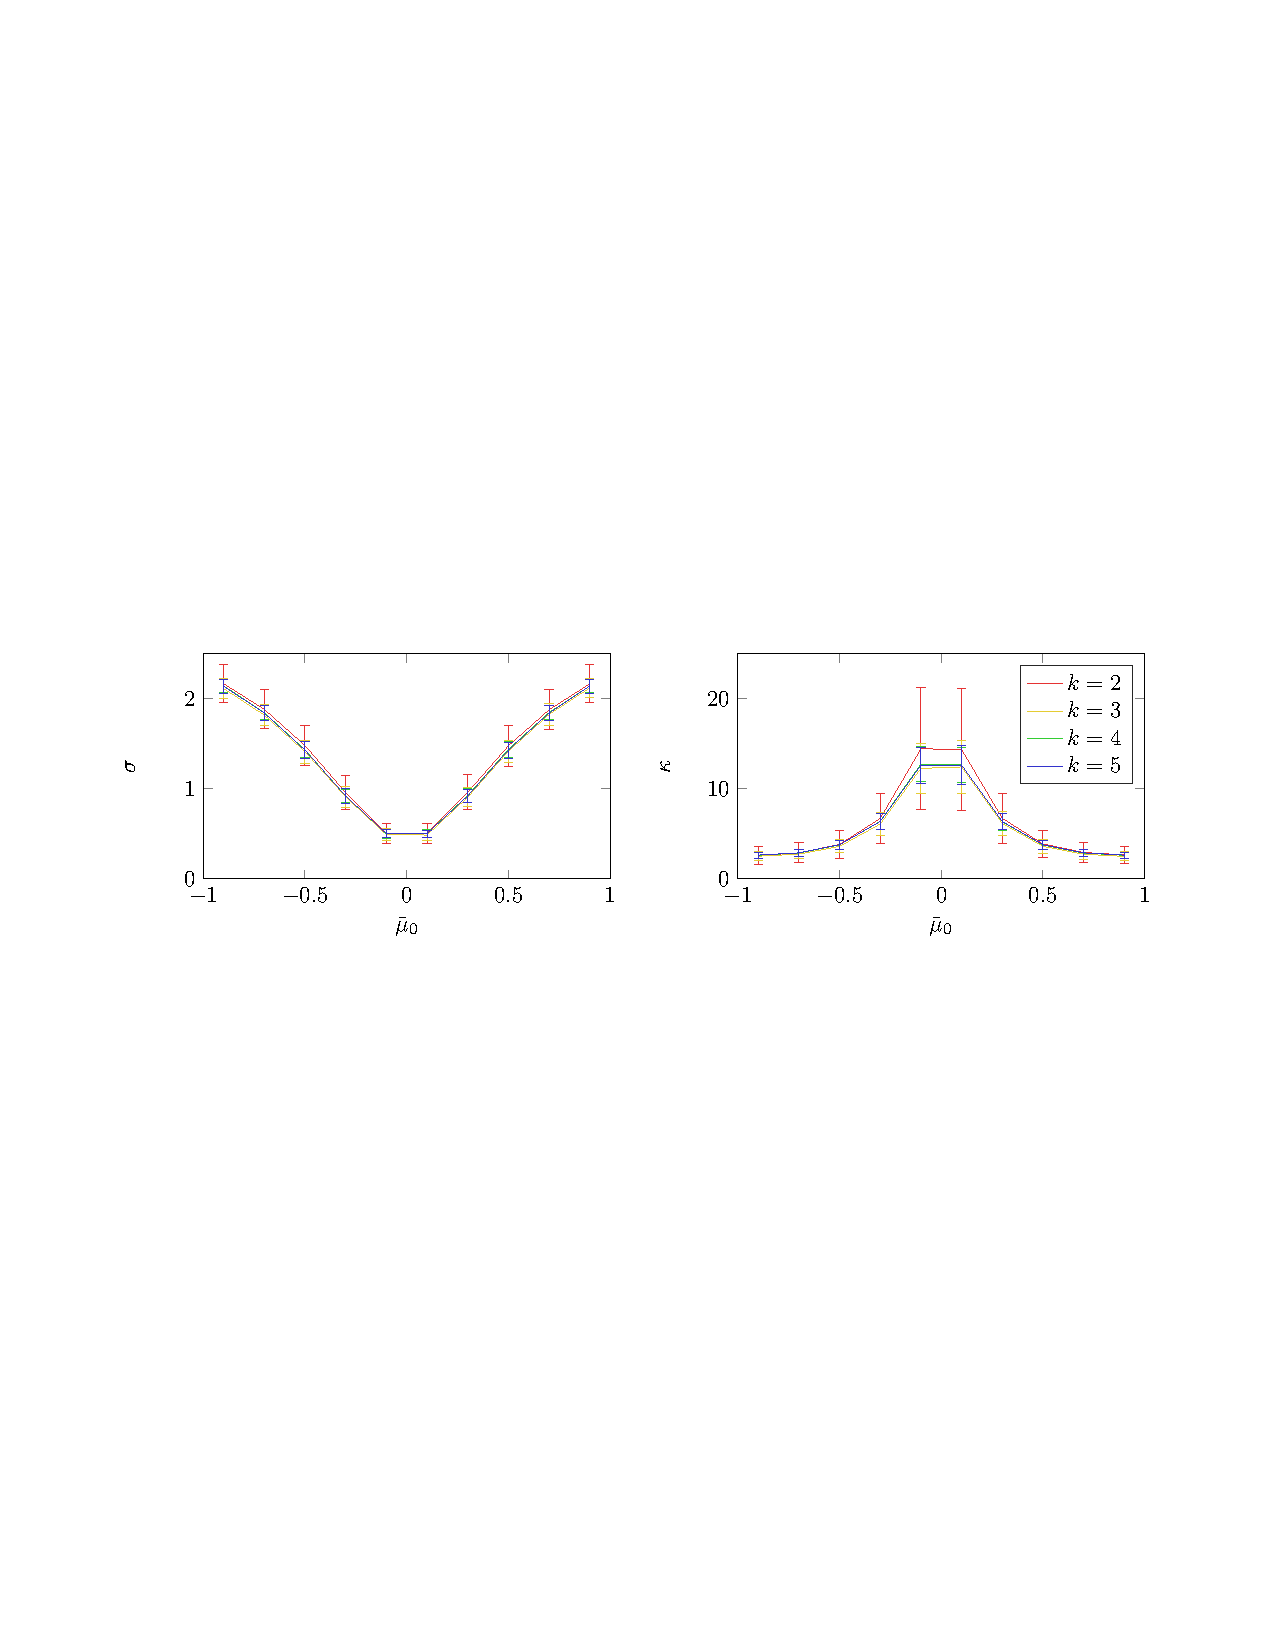
\includegraphics[width=\textwidth]{figures/appendix/theory/finitesizeplot2.pdf}
\caption{Finite size effects with $u_0=0.3$, $C_0=3$, $C_2=1$, $\sigma_0=1$, $\eta_0=20$.  Numerical averages are performed over 100 disorder realizations.}
\label{fig:AL_finitesize2plot}
\end{figure}

\begin{figure}[t]
\centering
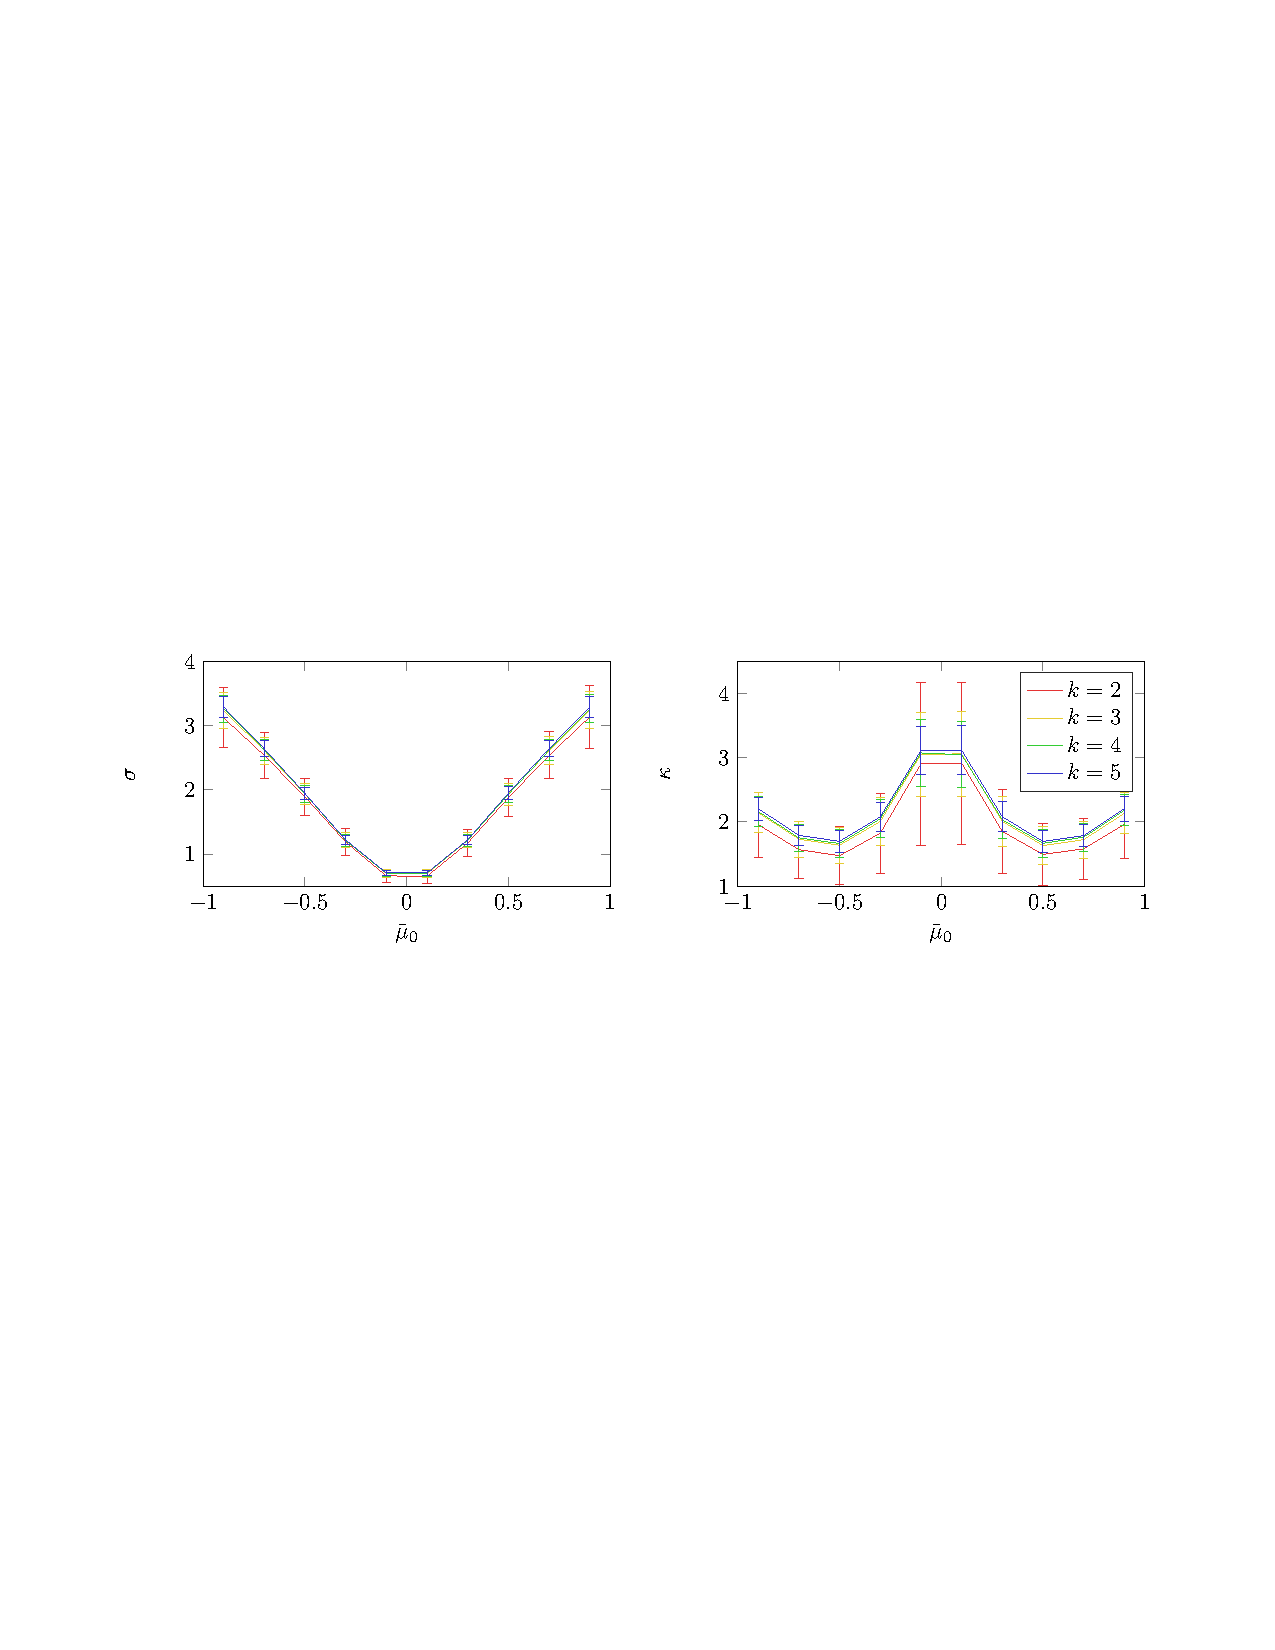
\includegraphics[width=\textwidth]{figures/appendix/theory/finitesizeplot1.pdf}
\caption{Finite size effects with $u_0=0.3$, $C_0=1$, $C_2=1$, $\sigma_0=1$, $\eta_0=1$.  Numerical averages are performed over 100 disorder realizations.}
\label{fig:AL_finitesizeplot}
\end{figure}


The other source of finite size effects is related to the finite number of grid points in our pseudospectral methods.   However, we expect standard exponential accuracy \cite{trefethen_spectral_2001} in the number of grid points per $\xi$, which we have taken to be at least 10 in all figures in the main text.   Numerical evidence suggests that our spectral methods have converged to within about 0.1--1\% of the correct answer by this relatively small number of grid points per $\xi$, depending on the precise equations of state used.  In the case of the experimentally relevant parameters used in Figure \ref{fig:AL_mainfig}, we see exponential convergence of our spectral methods with increasing grid points, with numerical error of only 0.1\% by the time the number of grid points per $\xi$ is 11, as shown in Figure \ref{fig:AL_spectralfig}.     This spectral convergence is dramatically faster in the weak disorder limit.

\begin{figure}[t]
\centering
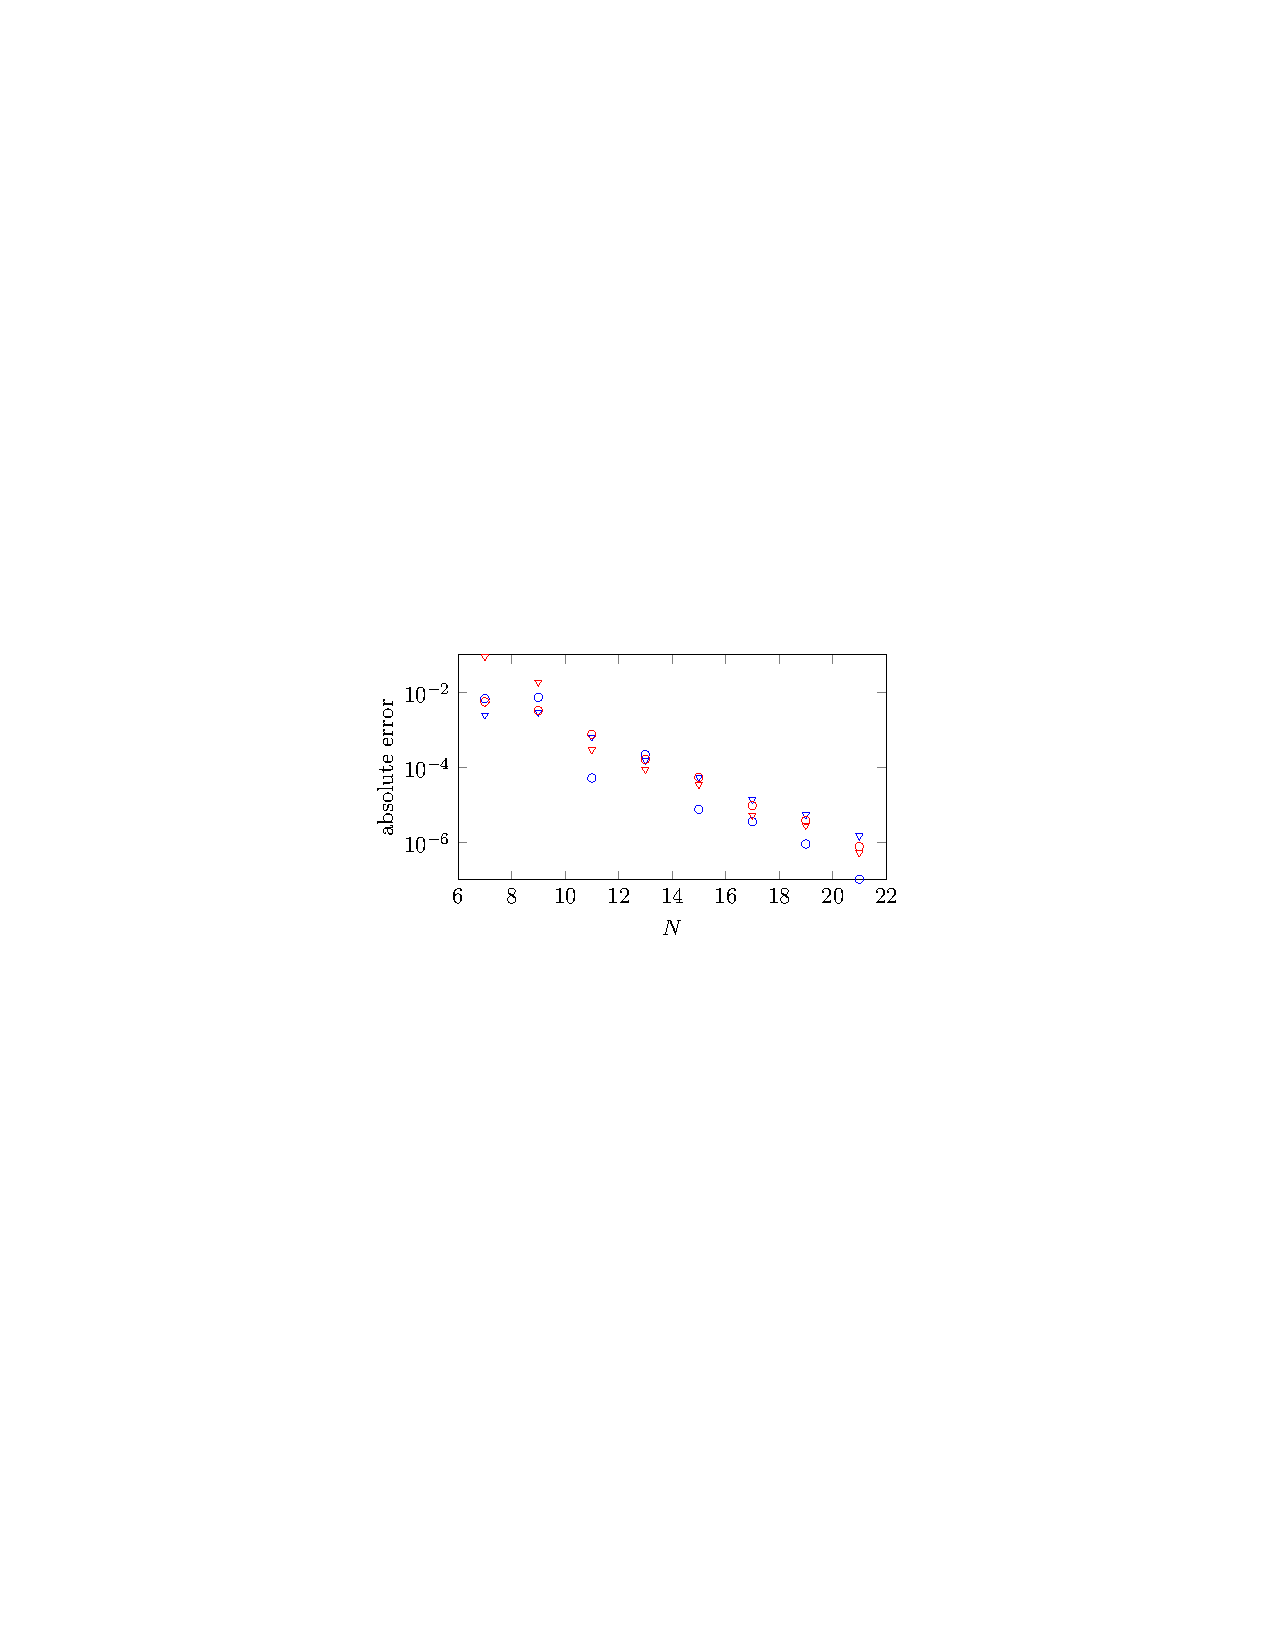
\includegraphics[width=3.3in]{figures/appendix/theory/spectralplot.pdf}
\caption{Exponential convergence of our pseudospectral code with an increasing number of grid points.  We computed $\kappa$ and $\sigma$ using our  code, employing the ``experimental" equations of state given in Figure \ref{fig:AL_mainfig},  and the disorder profile $\mu_0(x) = \bar\mu_0 + 2u\cos(2\pi x/L)\cos(2\pi y/L)$.   Red data points denote the error in $\kappa$, and blue points denote the error in $\sigma$.   Circles denote data at $\bar\mu_0 = 2u$, and triangles at $\bar\mu_0 = 0.4u$.  Absolute error is determined by (e.g.) $|\sigma(N)-\sigma(29)|/\sigma(29)$,  where we use the data points at $N=29$ as a reference point.}
\label{fig:AL_spectralfig}
\end{figure}

Methods are known to improve our simple algorithms, which can reduce both types of finite size effects discussed above.   Given the preliminary nature of the experiments to which we compare our simulations, we have found the numerical errors described above tolerable.

\subsection{Dimensional Analysis}
\newthought{We have performed numerical computations} in dimensionless units,   since we can trivially restore the units to our numerical results via dimensional analysis.   Setting $\hbar=k_{\mathrm{B}}=e=v_{\mathrm{F}}=T_0=1$ completely non-dimensionalizes the problem, while setting no dimensionless parameters to unity.    We can now trivially restore the units as follows:  \begin{subequations}\begin{align}
L &= \frac{\hbar v_{\mathrm{F}}}{k_{\mathrm{B}}T_0} \times L_{\mathrm{numerics}} \sim (100 \; \mathrm{nm}) \times L_{\mathrm{numerics}} \\
\mu &= k_{\mathrm{B}}T_0  \times \mu_{\mathrm{numerics}} \sim (5\; \mathrm{meV}) \times \mu_{\mathrm{numerics}}, \\
\sigma &= \frac{e^2}{\hbar}  \times \sigma_{\mathrm{numerics}} \sim (0.25\; \mathrm{k\Omega}^{-1}) \times \sigma_{\mathrm{numerics}}, \\
\alpha &= \frac{k_{\mathrm{B}}e}{\hbar}  \times \alpha_{\mathrm{numerics}} \sim \left(20\; \frac{\mathrm{nW}}{\mathrm{V}}\right) \times \alpha_{\mathrm{numerics}}, \\
\kappa &= \frac{k_{\mathrm{B}}^2T_0}{\hbar}  \times \kappa_{\mathrm{numerics}} \sim \left(0.1\; \frac{\mathrm{nW}}{\mathrm{K}}\right)  \times \kappa_{\mathrm{numerics}}.
\end{align}\end{subequations}
We have also noted the approximate scale of each important physical quantity in the problem for convenience.